\documentclass[minion]{homework651}
%% Feel free to add your own commonly used commands to this file.

\newcommand{\Reals}{\ensuremath{\mathbb R}}% Gives you a shortcut for writing the blackboard R for the real numbers - \RR
\newcommand{\Nats}{\ensuremath{\mathbb N}} % Gives you a shortcut for writing the blackboard N for the natural numbers - \NN
\newcommand{\Ints}{\ensuremath{\mathbb Z}} % Gives you a shortcut for writing the blackboard Z for the integer numbers - \ZZ
\newcommand{\Rats}{\ensuremath{\mathbb Q}} % Gives you a shortcut for writing the blackboard Q for the rational numbers - \QQ
\newcommand{\Cplx}{\ensuremath{\mathbb C}} % Gives you a shortcut for writing the blackboard C for the complex numbers - \CC

% Make better absolute value bars and the norm symbol
\newcommand{\abs}[1]{\left|#1\right|}
\newcommand{\norm}[1]{\left|\left|\,#1\,\right|\right|}

%% Now make some equivalents that some people may prefer.
\let\RR\Reals
\let\NN\Nats
\let\II\Ints
\let\CC\Cplx
\let\ZZ\Ints

%Add a shortcut for \rightarrow
\let\ra\rightarrow

%Add a \diam command for diameter
\newcommand{\diam}{\text{diam}}

\def\calB{\mathcal{B}}
\DeclareMathOperator{\Int}{\mathrm{Int}}
\usepackage{graphicx}
\usepackage{float}


\doclabel{Math F651: Homework 6}
\docdate{Due: March 1, 2023}
\docauthor{Stefano Fochesatto}

\begin{document}
\begin{problems}
    \problem
    Although quotient maps must take saturated open sets to open sets
    and saturated closed sets to closed sets, a quotient map need not be open or closed.  The point of this exercise is to see an example.
    
    Let $A$ be the set of points $(x,y)$ in $\Reals^2$ with $y=0$ or $x\ge 0$.  Let $\pi((x,y))=x$.
    Show that $\pi:A\rightarrow\Reals$ is a quotient map, but that it is neither open nor closed.
    \begin{proof} Let $A$ be the set of points $(x,y)$ is $\Reals^2$ with $y=0$ or $x\ge 0$.  Let $\pi((x,y))=x$. To prove that $\pi$ is a 
        quotient map we must show that $\pi$ is a continuous surjective map which takes saturated open sets to open sets.
        Clearly $\pi$ is a continuous surjection, since $\pi$ is simply $\pi_1|_A$ a restriction on the natural projection onto the first component of $\RR^2$. 
        Let $V \subseteq A$ be an closed saturated set, by definition there exists some $W \subseteq \Reals$ such that $V = \pi^{-1}(W)$. Let $\tilde{\RR} \subseteq A$
        be the set of points $(x,y)$ with $y=0$. Note $\RR$ is homeomorphic to $\tilde{\RR}$ and since $V \cap \tilde{\RR}$ is closed in $\tilde{\RR}$ by 
        the subspace topology induced by $A$, it follows that it's homeomorphic image $\pi(V)$ is closed in $\RR$. 
    \end{proof}
    
    \problem
    Let $\pi:X\rightarrow Y$ be a quotient map and let $A\subseteq X$
    be a saturated closed set or a saturated open set.  Show that $\pi|_A:A\rightarrow \pi(A)$
    is a quotient map.
    \begin{proof} Let $\pi:X\rightarrow Y$ be a quotient map and let $A\subseteq X$
        be a saturated closed set or a saturated open set. Now consider  $\pi|_A:A\rightarrow \pi(A)$. 
        Note that it is a continuous surjection, since $\pi$ was continuous and we've restricted it's codomain to $\pi(A)$. 
        Now suppose $V \subseteq \pi(A)$ such that $W = \pi|_A^{-1}(V)$ is open in $A$. Note that since $A$ has the subspace topology $W$ must be open 
        in $X$ and therefore since $\pi$ is a quotient map $\pi(W)$ is open in $Y$. Since $W \subseteq A$ it follows that $\pi|_A(W) = \pi|_A(\pi|_A^{-1}(V)) = V$ is open in $\pi(A)$.
    \end{proof}





    
    \problem Problem 3-14 Show that the real projective space $\PP^n$ is an n-manifold. [Hint: Consider the subsets $U_i \subseteq \RR^{n + 1}$ where $x_i = 1$.]
    
    \problem Problem 3-16 Let $X$ be the subset $(\RR \times \{0\}) \cup (\RR \times \{1\}) \subset \RR^2$. Define an equivalence relation on $X$ by declaring $(x, 0) \sim (x, 1)$
    if $x \neq 0$. Show that the quotient space $X/\sim$ is locally euclidean and second countable, but not Hausdorff.   
    
    Your solution should not be longer than a page.  Extra credit for the
    shortest correct solution.

    \problem
    No rigor please on this problem.  Just coherent explanations, and maybe a picture or two.
    \begin{subproblems}
    \item Define an equivalence class on $\Cplx$ where $z\sim w$ if there is $u\in S^1$ with
    $z=wu$.  The quotient space $\Cplx/\sim$ is a familiar topological space.  Name it.
     (``is'' means ``is homeomorphic to, of course''). 
    \begin{proof}
        We can see that the equivalence classes formed in the quotient space consist of $x \in \CC$ with the same magnitude (or norm), so naturally we can thing of $\CC/\sim$ as 
        being homeomorphic to the interval $[0, \infty)$. To show this It would be appropriate to use the Uniqueness of Quotient Spaces, let $q: \CC \to \CC/\sim$ be the natural 
        quotient map sending each element to its equivalence class. We would like to show that $f:\CC \to [0, \infty)$ defined by $f(a + bi) = \sqrt{a^2 + b^2}$ is a quotient map and makes the same 
        identifications as $q$.
    \end{proof}




    \item Define an equivalence class on $\Reals^2$ where $(x,y)\sim (x+1,-y)$ (along with all the relations then implied by transitivity).  The resulting quotient space is a familiar one.  Name it.
    \begin{proof}
        Note that the quotient space is homeomorphic to $M = [0, 1) \times \RR$, where each point in $M$ represents an equivalence class of points related by 
        $(x,y)\sim (x+1,-y)$. Some of these classes are illustrated below, 

        \begin{figure}[H]
          \begin{center}
            \caption{Mobius Strip}
            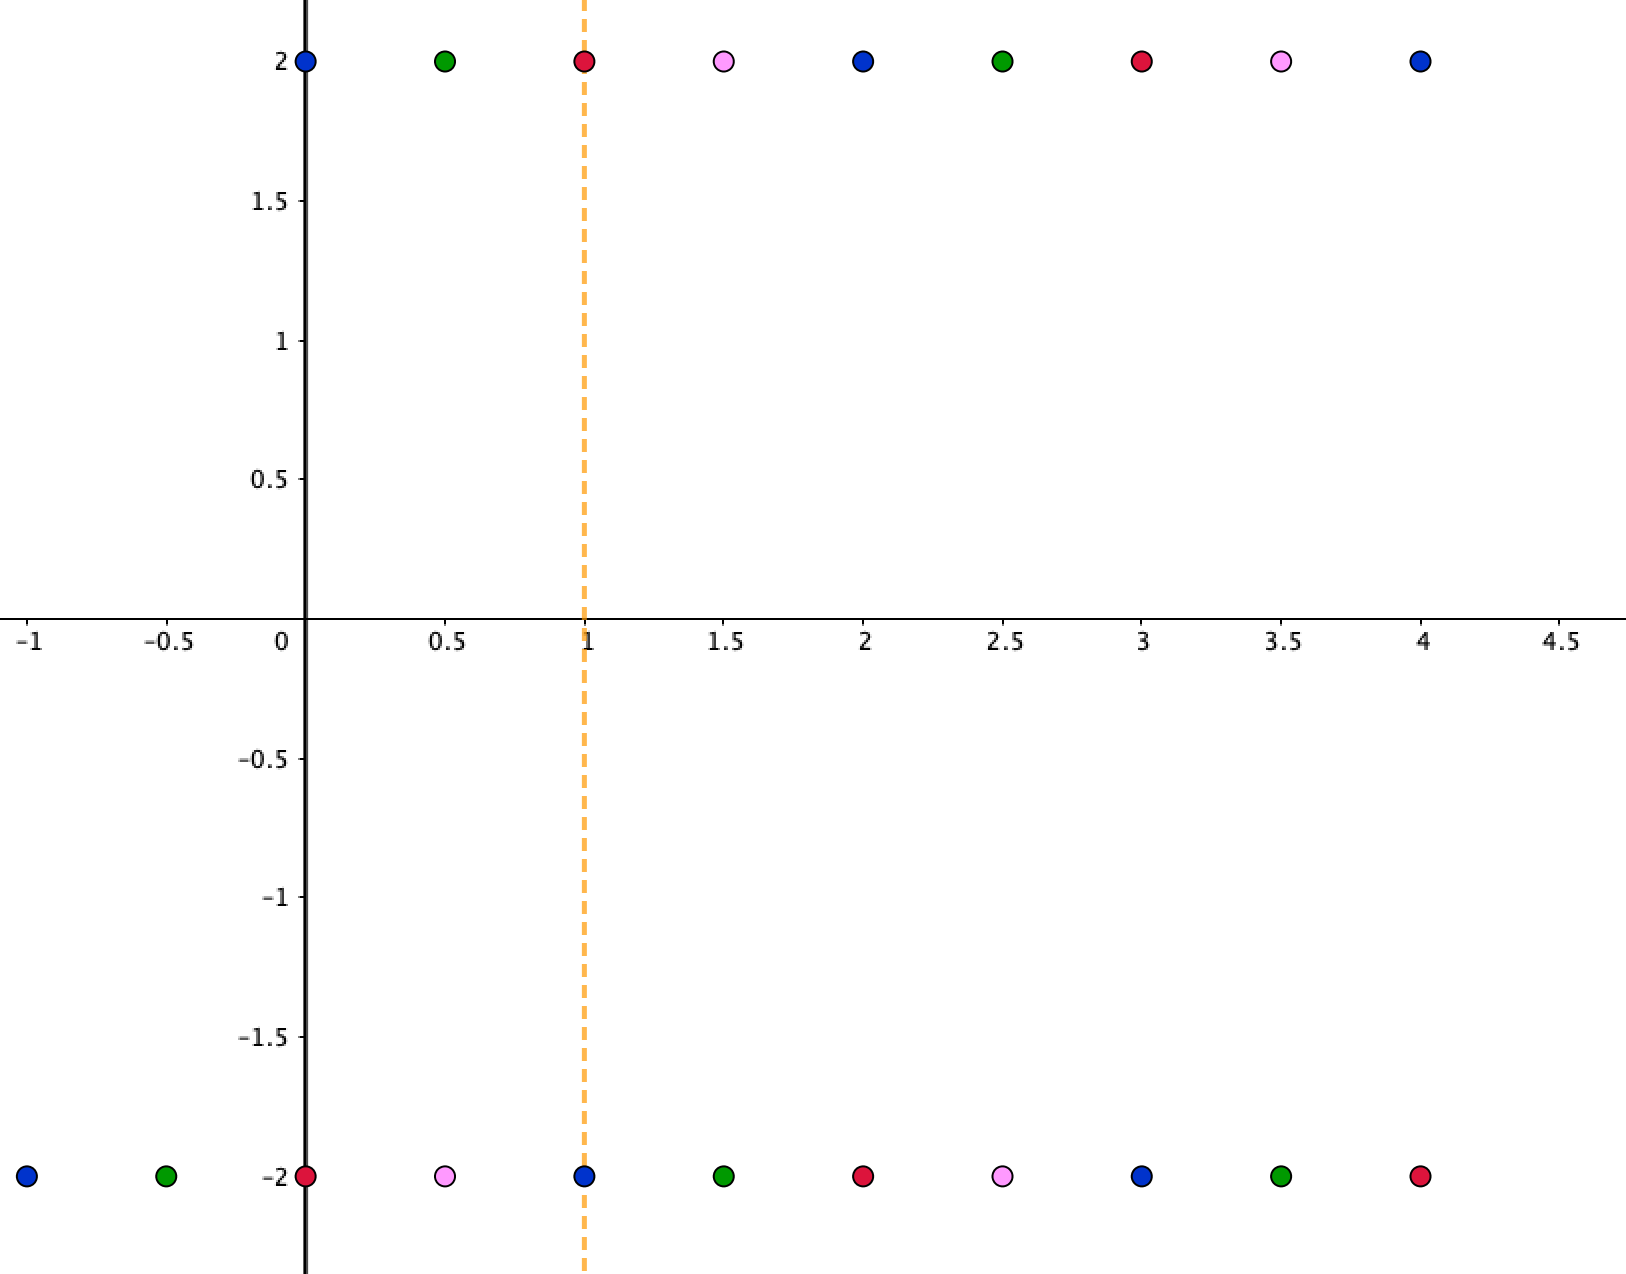
\includegraphics[width=.76\textwidth]{MOBIUS.png}
          \end{center}
        \end{figure}

        
    \end{proof}
    \end{subproblems}
    
    
    \problem
    Let $X=\Reals\times\{0,1\}$ and define an equivalence
    relation on $X$ by $(0,0)\sim(0,1)$.  Rigorously show that $X/\sim$
    is homeomorphic to the union of the $x$- and $y$-axes in the plane.
    \begin{proof} 
        Let $\RR^{xy} = \RR\times \{0\} \cup \{0\}\times\RR$ and consider the $q: X \to X/\sim$ be the natural projection sending each element of $X$ to its equivalence class. We will use the Uniqueness of Quotient
        spaces to show that $\RR^{xy}$ is homeomorphic to $X/\sim$, by constructing a quotient map $q^*: X \to \RR^{XY}$ which makes the same identifications as $q$.
        Let $q^*((x, y))$ be defined by, 
        \begin{equation*}
            q^*((x, y)) = \biggl\{\begin{array}{cc}
                (x, 0), & y = 0\\
                (0, x), & y = 1
              \end{array}\biggr\}.
        \end{equation*}
        Let $(x, y) \in \RR^{xy}$ and note that by definition either $x = 0$ or $y = 0$, without loss of generality let $x = 0$ now note that 
        for $(y, 1) \in X$ we know that $q^*((y, 1)) = (0, y) = (x, y)$. Hence $q^*$ is surjective. 

        Now note that $\{\Reals\times\{0\}, \Reals\times\{1\}\}$ form a finite closed cover for $X$. Let $q^*_0:\Reals\times\{0\} \to \RR\times \{0\}$ be defined by $q^*$
        restricting it's domain. Clearly $q^*_0$ is continuous as it becomes the identity map. Let $q^*_1:\Reals\times\{1\} \to \{0\}\times \RR$ be defined by restricting the domain of $q^*$.
        Note that $q^*_1 = \iota \circ \pi_1 $ where $\pi_1$ is the projection into the first component, and $\iota$ is the natural embedding into $\{0\}\times \RR$. Since $q^*_1$ is a composition of 
        continuous functions, $q^*_1$ is continuous. Since $q^*_1((0, 0)) = (0, 0) = q^*_0((0, 0))$ it follows by the glueing lemma that $q^*$ is a continuous map. 
   

        Now we will show that $q^*$ is a closed map. Let $C \subseteq X$ be a closed set note that $C = C_0 \cup C_1$ where $C_0$ and $C_1$ 
        are closed in $\Reals\times\{0\}$ and $\Reals\times\{1\}$ respectively. So it follows that that $q^*(C) = q^*_0(C_0) \cup q^*_1(C_1)$.  Clearly $q^*_0$ and $q^*_0$ are homeomorphisms, so they are closed maps, whose images in 
        $\RR^{xy}$ are closed, and thus $q^*_0(C_0)$ and $q^*_1(C_1)$ are closed in $\RR^{xy}$. Finally we can conclude that $q^*(C)$ is closed in $\RR^{xy}$ and that $q^*$ is a closed map. 

        Therefore $q^*$ is a quotient map. Note that $q((0, 0)) = q((0, 1))$ and evidently $q^*((0, 1)) = (0, 0) = q^*((0, 0))$ so $q$ and $q^*$
        make the same identifications and thus by the Uniqueness of the Quotient Spaces we know that there exists homeomorphism $f:  X/\sim \to \RR^{xy}$. 

    \end{proof}



    
    \problem Problem 4-1 Show that for $n > 1$, $\RR^n$ is not homeomorphic to any open subset of $\RR$. 
    \begin{proof}
       Let $n > 1$ and suppose $f: \RR^n  \to \RR$ is a homeomorphism. Let $y \in \RR$ and $x \in \RR^n$ such that $f(x) = y$. Since $f$
       is a homeomorphism it must them follow that $f^*: \RR^n - \{x\} \to \RR - \{y\}$ defined by $f^*(x) = f|_{\RR^n - \{x\}}$ is a homeomorphism as well. 
       However note that $\RR - \{y\}$ is a disconnected space while $\RR^n - \{x\}$, for $n > 1$ is still connected. 
    \end{proof}
    
    \problem \exercise{4-4} Prove that a topological space $X$ is disconnected if an only if there exists a nonconstant continuous function from $X$ to the 
    discrete space $\{0, 1\}$. 
    \begin{proof} $(\Rightarrow)$ Suppose a topological space $X$ is disconnected. Then by definition there exists nonempty, open $U, V \subseteq X$ such $U \cup V = X$ and $U\cap V = \emptyset$. 
        Define $f: X \to \{0, 1\}$ such that $f(x) = 1$ when $x \in U$ and $f(x) = 0$ when $x \in V$. This function is continuous. 
    \end{proof}
    \begin{proof} $(\Leftarrow)$ Suppose there exists a continuous function $f: X \to \{0, 1\}$. Note that $f^{-1}(\{0\}) \cap f^{-1}(\{1\}) = f^{-1}(\{0\} \cap \{1\}) = \emptyset$ and that $f^{-1}(\{0\}) \cup f^{-1}(\{1\}) = f^{-1}(\{0\} \cap \{1\}) = \emptyset$ and that $f^{-1}(\{0\} \cup \{1\}) = X$. 
        So therefore $X$ is disconnected. 
    \end{proof}


\end{problems}
\end{document}
